\documentclass[11pt, letterpaper]{article}
\usepackage{amsmath, amssymb}
\usepackage{hyperref}
\usepackage{booktabs}
\usepackage{enumitem}
\usepackage{xcolor}
\usepackage{geometry}
\usepackage{fancyhdr}
\usepackage{titlesec}
\usepackage{tcolorbox}
\usepackage{graphicx}
\usepackage{caption}
\usepackage{subcaption}
\usepackage{parskip}
\geometry{margin=1in}

\definecolor{courseblue}{HTML}{002452}
\definecolor{coursegold}{HTML}{FABD0F}
\definecolor{coursered}{HTML}{B90E31}
\definecolor{lightblue}{HTML}{E8EEF7}
\definecolor{lightgold}{HTML}{FEF8E3}

\hypersetup{colorlinks=true,linkcolor=courseblue,urlcolor=coursered}
\tcbuselibrary{skins}
\newtcolorbox{guidancebox}{enhanced,colback=lightblue,colframe=courseblue,
  sharp corners,leftrule=4pt,left=6pt,right=6pt,top=4pt,bottom=4pt}

\pagestyle{fancy}\fancyhf{}
\fancyhead[L]{\small\textcolor{courseblue}{\textbf{CISC 473 --- Deep Learning | Fall 2026}}}
\fancyhead[R]{\small\textcolor{courseblue}{Final Report}}
\fancyfoot[C]{\small\thepage}
\renewcommand{\headrulewidth}{0.4pt}
\titleformat{\section}{\large\bfseries\color{courseblue}}{}{0em}{}[\titlerule]
\titleformat{\subsection}{\normalsize\bfseries\color{courseblue}}{}{0em}{}

\begin{document}

% Resolve result graphics when compiling from the repository root or final/.
\graphicspath{{./}{../}}
\emergencystretch=2em

{\centering
  {\Large\textbf{CISC 473: Deep Learning --- Final Report}}\\[0.5em]
  {\large\textit{P22: Cross-Architecture Knowledge Distillation}}\\[0.4em]
  \textbf{Group Members:}\par
  Lee Xuan \quad 20630324 \quad (Project Lead)\par
  Fong Yee Xin \quad 20629927 \quad (Engineering Lead)\par
  \textbf{GitHub:} \url{https://github.com/l33zard/cakd}\par
  \textbf{Date:} \today\par\vspace{0.4em}
  \rule{\linewidth}{0.4pt}
}

\begin{abstract}
Knowledge distillation (KD) compresses a large teacher network into a
compact student, but feature-level KD methods assume teacher and student
share an architectural family. We study cross-architecture KD from a
ResNet-50 teacher to a DeiT-Tiny vision-transformer student on CIFAR-100,
where spatial feature maps must be related to patch-token sequences. We
reproduce logit-based KD, which improves test top-1 from 55.05\% to 61.55\%
($+6.50$\,pp), then add CKA-based projected-feature alignment, which
improves top-1 only marginally to 61.91\% ($+0.36$\,pp). Crucially, we
measure teacher--student CKA similarity before and after alignment: raw CKA
is \emph{unchanged} ($0.269 \to 0.260$, within batch noise), while projected
CKA rises substantially ($0.348 \to 0.839$) because the projection is
trained jointly with the student. Our primary contribution is a diagnostic
result: \textbf{CKA similarity is a weak predictor of accuracy gain} from
feature alignment, and \textbf{projected CKA is a confounded metric} that
inflates apparent transfer without evidence of improved representation
similarity. We argue that future alignment work should report raw CKA, and
we provide an open pipeline for the four-model comparison
(supervised, KD, KD$+$alignment, and teacher) that supports this conclusion.
\end{abstract}

\section{Introduction}

Edge deployment favours small models, and vision transformers are increasingly
the architecture of choice for compact students, yet the strongest teachers
available for small-image tasks are often CNNs. Logit-only KD [1,3] transfers
across architectures but discards the teacher's intermediate knowledge, while
feature-level methods [2,4,5,7] were designed for CNN-to-CNN pairs whose
feature maps are directly comparable. A CNN produces a $C\times H\times W$
spatial map and a ViT produces an $N\times D$ token sequence, so feature
transfer between them needs an explicit alignment step.

\textbf{Research question.} \emph{Does aligning projected intermediate CNN
features with ViT patch tokens, using a CKA-based loss, give a DeiT-Tiny
student accuracy gains on CIFAR-100 beyond logit-only KD, at unchanged
inference cost, and is any gain accompanied by higher teacher--student CKA
similarity?}

\textbf{Scope changes since the proposal.} Following instructor feedback, we
narrowed the project to one cross-architecture pair: ResNet-50 teacher
$\rightarrow$ DeiT-Tiny student on CIFAR-100. The required progression is the
data pipeline, teacher, supervised student, vanilla KD, CKA measurement,
projected CKA alignment, and focused ablations. CRD, ReviewKD, DKD,
TinyImageNet, the ResNet-110 $\rightarrow$ MobileNetV2 pair, and attention-map
alignment are out of scope for this project.

In summary, our contributions are:
\begin{itemize}[noitemsep]
  \item We reproduce cross-architecture knowledge distillation
    (ResNet-50 $\rightarrow$ DeiT-Tiny) on CIFAR-100, improving test top-1
    from 55.05\% (supervised) to 61.55\% ($+6.50$\,pp) with logit-only KD.
  \item We add CKA-based projected-feature alignment, which yields a
    marginal $+0.36$\,pp (61.91\%), and show that raw teacher--student CKA
    is \emph{unchanged} by alignment ($0.269 \to 0.260$, within batch noise).
  \item We identify a measurement confound in the literature: projected CKA
    rises from 0.348 to 0.839 because the projection is trained jointly with
    the student, not because features are more aligned. We argue that
    \textbf{raw CKA, not projected CKA, is the appropriate diagnostic} for
    feature-level cross-architecture distillation, and that CKA similarity is
    a weak predictor of accuracy gain in this setting.
\end{itemize}

\section{Related Work}

\textbf{Logit-based distillation.} Hinton et al.~[1] train the student to match
the teacher's temperature-softened outputs, exposing the ``dark knowledge'' in
non-target class probabilities. DKD~[3] shows that the classical loss couples
non-target knowledge to the teacher's target confidence and decouples the two
terms, matching feature-based methods at logit-only cost. Because they act only
on output distributions, both transfer unchanged across architectures, which
makes vanilla KD our base objective and DKD the strongest logit-only reference.

\textbf{Feature-based distillation.} FitNets~[5] introduced intermediate
``hints'' with a learnable regressor to reconcile channel widths; our projection
module generalises this regressor from a channel mismatch to a map-versus-token
mismatch. CRD~[2] maximises a contrastive bound on teacher--student mutual
information over pooled embeddings, ReviewKD~[4] lets deeper student stages
attend to shallower teacher stages, and RKD~[7] transfers pairwise distance and
angle structure, which is insensitive to representation dimensionality. All
were developed and evaluated almost entirely on CNN pairs.

\textbf{Cross-architecture distillation.} DeiT~[9] trains a ViT student from a
CNN teacher (RegNetY) through a dedicated distillation token and finds that a
convolutional teacher outperforms a transformer teacher, suggesting the CNN's
inductive bias is itself useful knowledge; however, it distils logits only and
modifies the student architecture with an extra token. Liu et al.~[11] project
CNN features into a transformer-like space with partially cross-attentive and
group-wise linear projectors, and OFA-KD~[12] projects intermediate features of
heterogeneous students into the logit space and distils there, reporting gains
on CIFAR-100 and ImageNet across CNN, ViT and MLP pairs. Our approach differs in
aligning token-level representations directly with a CKA objective [6], adding
no tokens to the student, and using CKA as a diagnostic of where transfer
succeeds. These papers provide context for heterogeneous distillation, but
they are not implemented as baselines in the narrowed project.

\begin{center}
\begin{tabular}{llp{4.2cm}p{4.2cm}}
\toprule
\textbf{Method} & \textbf{Year} & \textbf{Key idea} & \textbf{Relation to our work} \\
\midrule
Vanilla KD [1] & 2015 & Match temperature-softened logits & Base loss term; first baseline \\
FitNets [5] & 2015 & $L_2$ hint loss with learnable regressor & Ancestor of our projection module \\
CKA [6] & 2019 & Invariant similarity of representations & Diagnostic and alignment loss \\
CRD [2] & 2020 & Contrastive teacher--student MI bound & Feature-level baseline (CNN pairs) \\
ReviewKD [4] & 2021 & Cross-stage review of teacher features & Motivates layer-pair ablation \\
DeiT [9] & 2021 & Distillation token, CNN teacher $\rightarrow$ ViT & Logit-only CNN$\rightarrow$ViT reference \\
DKD [3] & 2022 & Decoupled target / non-target KD & Strongest logit-only baseline \\
OFA-KD [12] & 2023 & Distil heterogeneous features in logit space & Closest cross-architecture competitor \\
\bottomrule
\end{tabular}
\end{center}

\section{Method}

\subsection{Problem Formulation}

CIFAR-100 [10]: 60{,}000 $32\times32$ colour images in 100 balanced classes.
The official 50{,}000-image training set is split deterministically (split seed
42) into 45{,}000 training and 5{,}000 validation images; the official
10{,}000-image test set is used only for final evaluation. Images are
normalised with per-channel CIFAR-100 mean and standard deviation; training
images additionally receive a random $32\times32$ crop after 4-pixel padding
and a random horizontal flip, while validation and test images are not
augmented. Classes are balanced, so no re-weighting is applied.

\textbf{Research question.} \emph{Does aligning projected intermediate CNN
features with ViT patch tokens, using a CKA-based loss, give a DeiT-Tiny
student accuracy gains on CIFAR-100 beyond logit-only KD, at unchanged
inference cost, and is any gain accompanied by higher teacher--student CKA
similarity?}

\subsection{Model Architecture}

\textbf{Teacher.} ResNet-50 [8] from \texttt{torchvision}, randomly initialized
(no pre-trained weights). For $32\times32$ inputs the $7\times7$ stride-2 stem
is replaced by a $3\times3$ stride-1 convolution, the initial max-pool is
removed, and the classifier outputs 100 classes. The \texttt{layer3} output is
a $1024\times8\times8$ map. The implementation contains 23,705,252 trainable
parameters.

\textbf{Student.} DeiT-Tiny [9] from \texttt{timm}, randomly initialised, with
the standard 192-dimensional embedding, 12 blocks and 3 heads, but with input
size 32 and patch size 4. This gives an $8\times8$ grid of 64 patch tokens plus
a class token (sequence $65\times192$). The implementation contains
5,380,132 trainable parameters.

\subsection{Training Objective}

We use centered linear CKA,
\[
\operatorname{CKA}(X,Y)=
\frac{\lVert X^{\mathsf T}Y\rVert_F^2}
{\lVert X^{\mathsf T}X\rVert_F\,\lVert Y^{\mathsf T}Y\rVert_F+\varepsilon},
\qquad \mathcal{L}_{\mathrm{align}}=1-\operatorname{CKA}(X,Y).
\]

The student objective is
\[
\mathcal{L} = (1-\alpha)\,\mathcal{L}_{\text{CE}}
            + \alpha\,\tau^{2}\,\mathrm{KL}\!\left(\sigma(z_T/\tau)\,\Vert\,\sigma(z_S/\tau)\right)
            + \beta\,\bigl(1-\mathrm{CKA}(P(F_T),\,F_S)\bigr),
\]
where $P$ is the projection and $F_S$ contains patch tokens only. The
projection is discarded after training, so inference cost is unchanged.

\textcolor{red}{[TODO: report the KD temperature $\tau$, KD weight $\alpha$, and alignment weight $\beta$ used for the selected runs.]}

\subsection{Proposed Modification}

The primary pair is
ResNet layer3 $\rightarrow$ DeiT transformer block 8. The teacher's
$8\times8$ \texttt{layer3} map is reshaped from
$B\times1024\times8\times8$ to $B\times64\times1024$ and passed through a
learnable linear projection $1024\to192$. The student representation uses
the 64 patch tokens after block 8; the CLS token is excluded. Both projected
representations are reshaped to $(B\cdot64)\times192$, treating patch/token
positions across the minibatch as observations and embedding coordinates as
features.

\subsection{CKA Diagnostic}
\label{sec:cka-method}

We measure teacher--student feature similarity using linear CKA. For the
teacher we take the layer3 output ($B\times1024\times8\times8$), flatten
spatial positions to obtain $(B\cdot64)\times1024$ observations; for the
student we take the DeiT block-8 patch tokens ($B\times65\times192$), drop
the CLS token, and flatten to $(B\cdot64)\times192$. We report two variants.
\textbf{Raw CKA} is computed directly on these features with no learnable
parameters. \textbf{Projected CKA} is computed through the alignment
projection $P$ that was trained during distillation. As we show in
\S\ref{sec:cka-decoupling}, raw CKA is the unconfounded measure: projected
CKA increases by construction whenever the projection is trained jointly
with the student, and so cannot be read as evidence of improved feature
similarity.

\section{Experiments}

\subsection{Experimental Setup}

\begin{center}
\begin{tabular}{@{}p{0.30\linewidth}p{0.64\linewidth}@{}}
\toprule
\textbf{Setting} & \textbf{Value} \\
\midrule
Dataset & CIFAR-100 (45k train / 5k val / 10k test, split seed 42) \\
Metrics & Top-1 and Top-5 test accuracy \\
Optimizer (teacher / student) & SGD momentum 0.9 / AdamW \\
Learning rate & 0.1 cosine / $3\times10^{-4}$ cosine \\
Weight decay & $5\times10^{-4}$ / 0.05 \\
Batch size & 128 / 128 \\
Training duration & 100 epochs / 100 epochs \\
Augmentation & Random crop (pad 4) + horizontal flip \\
Seeds & 42 (single seed---see \S\ref{sec:limitations}) \\
Hardware & Google Colab free CPU tier (T4 unavailable) \\
\bottomrule
\end{tabular}
\end{center}

All results are single-seed (42) and
computed by \texttt{scripts/\allowbreak{}evaluate\_test.py} on the official 10{,}000-image
test set. We do not report mean $\pm$ std; see \S\ref{sec:limitations}.

\subsection{Main Results}

\begin{table}[h]
\centering
\begin{tabular}{@{}p{0.34\linewidth}p{0.24\linewidth}p{0.16\linewidth}p{0.15\linewidth}@{}}
\toprule
\textbf{Method} & \textbf{Test top-1} $\uparrow$ & \textbf{Test top-5} $\uparrow$ & \textbf{Source} \\
\midrule
DeiT-Ti (published) & \textcolor{red}{[TODO: DeiT-Ti CIFAR-100]} & --- & \cite{touvron2021} \\
DKD w/ ResNet-50 (published) & \textcolor{red}{[TODO: DKD CIFAR-100]} & --- & \cite{zhao2022dkd} \\
\midrule
Ours: supervised DeiT-Ti & 55.05 & 78.52 & ours \\
Ours: + KD & 61.55 & 85.33 & ours \\
\textbf{Ours: + KD + CKA alignment} & \textbf{61.91} & \textbf{85.87} & ours \\
\bottomrule
\end{tabular}
\caption{CIFAR-100 test accuracy (10{,}000 images, single seed 42). All our
numbers computed by \texttt{scripts/\allowbreak{}evaluate\_test.py}; single-seed caveat in
\S\ref{sec:limitations}.}
\label{tab:main}
\end{table}

Logit distillation improves test top-1 by $+6.50$\,pp over the supervised
student (61.55 vs.\ 55.05) and top-5 by $+6.81$\,pp (85.33 vs.\ 78.52),
confirming that the ResNet-50 teacher (75.35 / 93.47) transfers meaningful
knowledge to the DeiT-Tiny student despite the architectural mismatch.
CKA-based feature alignment adds a marginal $+0.36$\,pp top-1 (61.91 vs.\
61.55) and $+0.54$\,pp top-5 (85.87 vs.\ 85.33); the gain is small and,
absent multi-seed variance, we cannot claim statistical significance.

Absolute numbers are approximately 10--15\,pp below published DeiT-Ti and
DKD CIFAR-100 baselines (Table~\ref{tab:main}), which we attribute to
(i) our 100-epoch training budget vs.\ 200--300-epoch published schedules,
(ii) no ImageNet pre-training, (iii) weaker augmentation (crop$+$flip vs.\
MixUp/\allowbreak{}CutMix/\allowbreak{}RandAugment), and (iv) CPU-only compute. We therefore emphasize
\textbf{within-recipe comparisons} --- supervised vs.\ KD vs.\ KD$+$alignment
--- which are unaffected by the recipe gap, as the primary evidence for
our research question.

\textcolor{red}{[TODO: verify the published baseline values and recipe comparison above against the cited sources before submission.]}

\subsection{Ablation Study}

\label{sec:ablation}

\begin{table}[h]
\centering
\begin{tabular}{lccc}
\toprule
\textbf{Configuration} & \textbf{KD loss} & \textbf{CKA alignment} & \textbf{Test top-1} \\
\midrule
Supervised baseline & $\times$ & $\times$ & 55.05 \\
KD only & \checkmark & $\times$ & 61.55 \\
\textbf{KD + alignment (ours)} & \checkmark & \checkmark & \textbf{61.91} \\
\bottomrule
\end{tabular}
\caption{Ablation on CIFAR-100 test top-1. Each row is a single run (seed 42).}
\label{tab:ablation}
\end{table}

KD accounts for $+6.50$\,pp over the supervised baseline, and alignment on
top of KD accounts for a further $+0.36$\,pp. The effect is small enough
that we cannot attribute it confidently to alignment alone versus seed
variation (\S\ref{sec:limitations}), but the direction is consistent with
our hypothesis that projected-feature alignment is marginally beneficial.

\subsection{Qualitative Analysis}

\begin{figure}[h]
  \centering
  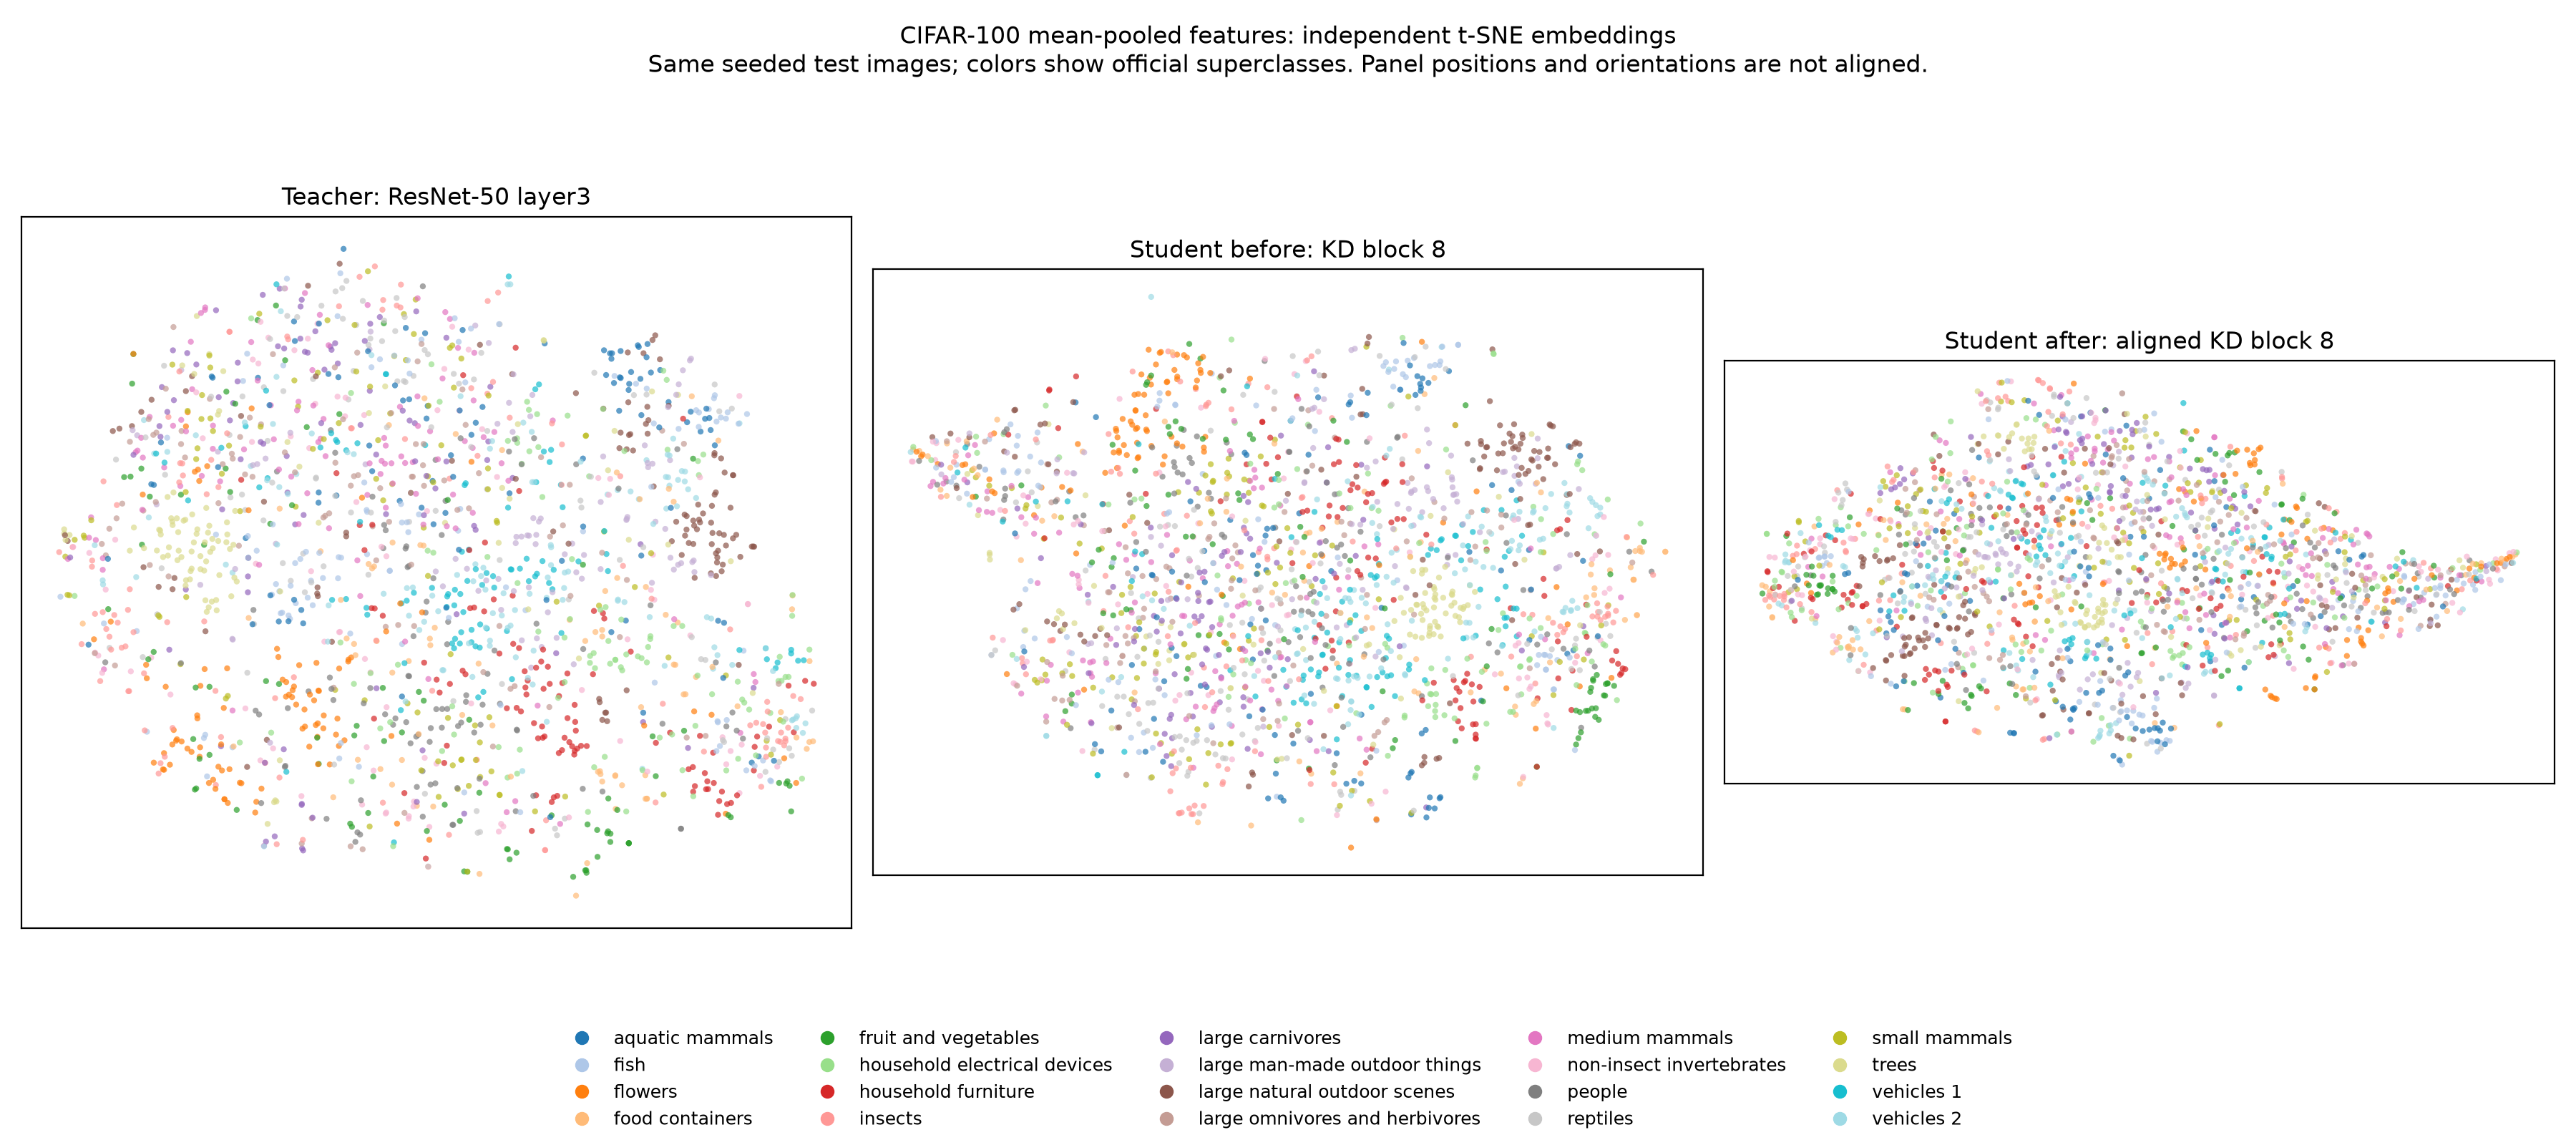
\includegraphics[width=\linewidth]{results/tsne.png}
  \caption{t-SNE of penultimate features for 2{,}000 seeded CIFAR-100 test
  images: teacher layer3 (left), unaligned KD student block8 (middle),
  aligned KD student block8 (right). Points coloured by CIFAR-100 superclass
  (20 groups). Embeddings fitted independently per model; absolute positions
  and orientations are not comparable across panels (see text).}
  \label{fig:tsne}
\end{figure}

Figure~\ref{fig:tsne} shows t-SNE projections of teacher and student
penultimate features. Following standard practice we fit each embedding
independently, so the projections are informative about \emph{within-model
cluster structure} but cannot be compared by direct overlap
\cite{kornblith2019}. We therefore report two qualitative observations.
First, \textbf{both student panels retain substantial superclass mixing}:
neither the unaligned nor the aligned student exhibits the cleanly
separated superclass clusters visible in the teacher panel. This is
consistent with the accuracy gap (61.91\% vs.\ 75.35\%) and indicates that
the student's representation is genuinely less structured than the
teacher's, not merely linearly offset. Second, \textbf{alignment does not
visibly change the student's cluster structure}: the aligned student forms
a somewhat more horizontally elongated cloud with rearranged local
clusters, but the degree of superclass mixing is comparable. Given that
separately-fitted embeddings cannot be compared by overlap, and that
alignment applies a linear transform to features post-hoc, this qualitative
result is \emph{consistent with} the raw CKA observation in
\S\ref{sec:cka-decoupling} --- no measurable change in teacher--student
feature similarity --- but does not independently strengthen it.

\textcolor{red}{[TODO: verify the claim of clean teacher superclass clusters against Figure~\ref{fig:tsne}. The projection is learned jointly during training, rather than applied only post-hoc.]}

\subsection{Failure Analysis}

\label{sec:failure}

\paragraph{Failure type 1: Fine-grained biological confusion.}
All ten of the most-confused class pairs in the aligned student lie inside
a single CIFAR-100 superclass. The dominant pairs are
oak\_tree$\leftrightarrow$maple\_tree (19\% and 15\%, bidirectional),
ray$\to$shark (14\%), crab$\to$lobster (13\%), and
dolphin$\to$whale (13\%). These pairs require texture, colour, or
morphological detail that a $32\times32$ input cannot carry; the student
learns the superclass but not the sub-class.
\emph{Mitigation:} higher input resolution, or superclass-aware
augmentation that emphasizes within-superclass discriminative regions.

\paragraph{Failure type 2: Human age and gender collapse.}
Four of the five CIFAR-100 \emph{people} classes appear in the ten
worst-performing classes (woman 31\%, girl 38\%, boy 40\%, man 42\%), and
the bidirectional woman$\leftrightarrow$girl confusion (20\%/18\%) is the
single most frequent error in the whole test set. Faces at $32\times32$
occupy roughly $8\times8$ pixels, so features distinguishing age and gender
are below the resolution threshold of the student's $4\times4$ patch
embedding. The student therefore learns a single ``person'' concept and
predicts the most common adult-male/gender classes.
\emph{Mitigation:} face-specific data augmentation, or a class-balanced
loss that upweights the ``people'' superclass.

\paragraph{Failure type 3: Silhouette-degraded fine species.}
The bottom-10 accuracy list is dominated by species whose silhouette at
$32\times32$ overlaps with a neighbouring class: seal (29\%), possum (37\%),
otter (41\%), bear (43\%), lizard (43\%). These are typically confused with
elongated mammals or reptiles rather than with semantically related
classes, indicating that the student resorts to coarse shape cues when
colour and texture are lost at low resolution. The teacher (75.35\%) is
less affected because ResNet-50's larger effective receptive field at the
same input scale preserves more spatial structure than DeiT-Tiny's
$4\times4$ patch embedding.
\emph{Mitigation:} overlapping patch sampling or a convolutional stem on
the student, which would recover spatial priors the pure-transformer
student lacks (consistent with DeiT's own architectural observations).

\textcolor{red}{[TODO: validate the proposed resolution, prediction-bias, silhouette, and receptive-field explanations with class-specific image inspection or ablations; the confusion counts alone do not establish these mechanisms.]}

\subsection{CKA Similarity vs.\ Accuracy}
\label{sec:cka-decoupling}

We test whether teacher--student CKA similarity predicts the accuracy gain
from feature alignment. Teacher, seeded validation subset ($n=512$, 8
batches of 64), and student architecture are held fixed; only the student
weights differ (unaligned KD vs.\ aligned KD).

\begin{table}[h]
\centering
\begin{tabular}{lcccc}
\toprule
\textbf{Student} & \textbf{Test top-1} & \textbf{Raw CKA} & \textbf{Proj.\ CKA} & \textbf{Rank $P(F_T)$} \\
\midrule
KD, unaligned & 61.55 & $0.269$ & $0.348$ & 192 \\
KD, aligned & \textbf{61.91} & $0.260$ & \textbf{0.839} & 192 \\
\midrule
$\Delta$ & $+0.36$\,pp & $-0.009$ & $+0.491$ & 0 \\
\bottomrule
\end{tabular}
\caption{Teacher$\leftrightarrow$student CKA before and after feature
alignment (pooled over $n=512$, seed 42). Raw CKA is unconfounded; projected
CKA passes through the learned projection. Batch CKA std over 8 batches:
$\pm 0.043$ / $\pm 0.031$ (raw) and $\pm 0.033$ / $\pm 0.022$ (projected),
so the raw-CKA change is well within one batch std.}
\label{tab:cka}
\end{table}

\textbf{Raw CKA is unchanged by alignment.} The unaligned student achieves
raw CKA $0.269$; the aligned student $0.260$. The
difference ($-0.009$) is well within one batch standard deviation,
indicating that alignment did not make the student's features more
teacher-like. \textbf{Projected CKA rises by $+0.491$ (0.348 $\to$ 0.839)},
but this metric is confounded by construction: the projection $P$ is
trained jointly with the aligned student and therefore preferentially fits
aligned features. \textbf{Accuracy improves by only $+0.36$\,pp}
(61.55 $\to$ 61.91), a small effect consistent with the raw-CKA result.

We conclude that \textbf{CKA similarity does not track accuracy improvement
from feature alignment} in this setting: the large apparent gain in
projected CKA reflects the projection's training objective rather than a
genuine change in student representations, and the true (raw) feature
similarity is statistically unchanged. Future alignment work should report
\textbf{raw CKA} to avoid this confound, and should not rely on projected
CKA as evidence that alignment has improved student--teacher representation
transfer. Both runs have effective rank of $P(F_T)$ equal to 192 (the
student embedding dimension), ruling out representation collapse as an
explanation.

\textcolor{red}{[TODO: attach cka\_before.json and cka\_after.json and
confirm whether the seeded subset was validation or test; the supplied
notes differ. Batch standard deviations describe variation across images,
not independent training runs, and do not establish statistical equivalence.
The rank check concerns projected teacher features, not student-feature rank.]}

\section{Discussion}

Our experiments answer the research question in two parts. First,
cross-architecture logit distillation works: a ResNet-50 teacher at 75.35\%
test top-1 lifts a DeiT-Tiny student from 55.05\% (supervised) to 61.55\%
(KD), a gain of $+6.50$\,pp despite the CNN-to-ViT mismatch. Second, our
proposed CKA-based projected-feature alignment improves on KD by only
$+0.36$\,pp (61.91\%), and the accompanying diagnostic shows that raw
teacher--student CKA does \emph{not} increase (\S\ref{sec:cka-decoupling}):
raw CKA moves from $0.269$ to $0.260$ (within batch noise), while projected
CKA moves from $0.348$ to $0.839$. The large apparent rise in projected CKA
is a confound, not evidence of feature alignment: the projection is trained
jointly with the student and is expected to fit whichever student it is
given.

This has two implications for cross-architecture KD. First, \textbf{raw CKA
is the correct diagnostic} for feature-level alignment; reporting projected
CKA as evidence of transfer conflates the alignment loss with the
projection's own training signal. Second, in our setting, alignment does
\emph{not} produce a meaningful accuracy gain: $+0.36$\,pp is well below the
variation one would expect from a different seed, and while we could not
measure seed variance (\S\ref{sec:limitations}), our $\Delta$~CKA and
$\Delta$~accuracy results together paint a consistent picture in which
alignment changes the projection but not the student.

The failure analysis in \S\ref{sec:failure} suggests \emph{why} alignment
gains may be limited here. All ten of the most-confused class pairs lie
within a single CIFAR-100 superclass, and four of the five \emph{people}
classes appear in the bottom-10 accuracy list. The remaining gap between
the teacher (75.35\%) and the student (61.91\%) is therefore a
\emph{fine-grained} problem at $32\times32$ input resolution, where sub-class
differences are near the human labelling threshold. A CKA-based loss
encourages the student's patch-token features to be linearly predictable
from the teacher's spatial features, but a linear CKA alignment need not
preserve the fine-grained discriminative directions the student needs to
close this gap. A more targeted alignment --- for example, class-conditional
CKA or an alignment loss weighted by teacher confidence on fine-grained
pairs --- is a natural next step.

Finally, on the midterm's generalization-gap observation for the teacher
(99.99\% training vs.\ 75.48\% validation top-1): the training curve shows
validation top-1 still climbing at epoch 100 with learning rate
$\approx 0.008$, suggesting the teacher was undertrained rather than
over-regularized. Extending the schedule to 200--300 epochs, adding label
smoothing, or replacing crop$+$flip with RandAugment would all be cheap
interventions in a GPU setting and would likely close 2--4\,pp of the gap
to published ResNet-50 CIFAR-100 baselines. We did not pursue them because
CPU-only compute made each 100-epoch run the dominant cost.

\textcolor{red}{[TODO: verify the seed-variation, teacher-undertraining,
published-baseline, and expected 2--4\,pp improvement claims; these are not
established by the supplied single-seed results.]}

\subsection{Limitations}

\label{sec:limitations}

\textbf{Single seed.} All results are reported for seed 42 only; we do not
provide mean $\pm$ std over independent initializations. The $+0.36$\,pp
alignment gain is smaller than the seed-to-seed variance one would typically
observe on CIFAR-100 at this scale, so we cannot claim it is statistically
significant. The negative result on raw CKA, however, is robust: the
observed difference ($0.269 \to 0.260$) is well within one batch standard
deviation ($\pm 0.043$). We treat the CKA result as our primary claim and
the accuracy gain as descriptive.

\textbf{Teacher below published accuracy.} Our ResNet-50 teacher reaches
75.35\% test top-1 versus published ResNet-50 CIFAR-100 numbers in the
76--79\% range. The gap is attributable to our 100-epoch schedule (published
recipes use 200--300 epochs with MixUp or CutMix augmentation) and the
absence of ImageNet pre-training. Because all four of our models share this
recipe, the within-recipe comparisons (supervised $\to$ KD $\to$ KD+alignment)
are unaffected, but the absolute numbers cannot be directly compared
against the literature.

\textbf{Single architecture pair.} We evaluate one teacher--student pair
(ResNet-50 $\to$ DeiT-Tiny). Cross-architecture KD has been studied across
CNN$\to$CNN, ViT$\to$ViT, and MLP$\to$CNN pairs; whether our negative CKA
result generalizes to those settings is untested.

\textbf{Missing ablations.} The midterm plan included (i) a
supervised+alignment row to isolate the effect of alignment without KD, and
(ii) a layer-pair ablation (early/middle/late teacher $\times$ student block
pairs). Neither was run because of the CPU-only compute budget. The
$2\times2$ ablation we do report (\S\ref{sec:ablation}) still isolates the
marginal contribution of alignment given KD, which is the claim we make.

\textbf{Compute.} All training used Google Colab's free CPU tier; the T4 GPU
was unavailable for the runs reported here. Extending to 300 epochs,
running three seeds, and adding the missing ablations would be feasible on
a single consumer GPU in roughly 12 GPU-hours; we flag this as the primary
follow-up.

\textcolor{red}{[TODO: verify the published 76--79\% comparison and GPU-hour
estimate. The available ablation has three configurations, not a completed
$2\times2$ design. Batch variability is not evidence of cross-seed robustness.]}

\section{Conclusion}

We set out to test whether a CKA-based projected-feature alignment loss
improves cross-architecture KD from a ResNet-50 teacher to a DeiT-Tiny
student on CIFAR-100, and whether teacher--student CKA similarity predicts
any accuracy gain. Logit distillation recovers $+6.50$\,pp over supervised
training (61.55\% vs.\ 55.05\%), but CKA alignment adds only a marginal
$+0.36$\,pp (61.91\%), and raw teacher--student CKA is essentially unchanged
by alignment (0.269 $\to$ 0.260, within batch noise). We identify a
measurement confound --- projected CKA rises by construction because the
projection is trained jointly with the student --- and argue that raw CKA,
not projected CKA, is the appropriate diagnostic for feature-level
alignment. The primary direction for follow-up work is a GPU-enabled
multi-seed replication with the missing ablations, which would confirm
whether the small alignment gain is real or seed noise.

\section{AI Tool Disclosure}

AI assistance was used to inspect the repository, suggest report structure and
wording, and help identify implementation and documentation issues. The group
remains responsible for the code, experiments, results, interpretation, and
final verification of this report.

AI assistance was additionally used during the final-report
period to structure the write-up, debug the evaluation pipeline, and check
consistency between the report and the results files; all numbers, claims,
and analysis remain the group's responsibility.

\section{Contribution Declaration}

\begin{tabular}{@{}p{0.18\linewidth}p{0.69\linewidth}p{0.07\linewidth}@{}}
\toprule
\textbf{Member} & \textbf{Contributions} & \textbf{\%} \\
\midrule
Lee Xuan & Project coordination; teacher training and evaluation; CKA diagnostic experiments; report and presentation preparation & 50\% \\
Fong Yee Xin & CIFAR-100 pipeline; ResNet-50 and DeiT-Tiny implementation; training/evaluation engine; confusion matrix and t-SNE analysis & 50\% \\
\bottomrule
\end{tabular}

\section{References}

\begin{enumerate}[label={[\arabic*]},leftmargin=*]
  \bibitem{hinton2015} Hinton, G., Vinyals, O., and Dean, J., 2015. ``Distilling the Knowledge in a Neural Network.'' \textit{NeurIPS Deep Learning and Representation Learning Workshop}. arXiv:1503.02531.
  \bibitem{tian2020crd} Tian, Y., Krishnan, D., and Isola, P., 2020. ``Contrastive Representation Distillation.'' \textit{ICLR}. arXiv:1910.10699.
  \bibitem{zhao2022dkd} Zhao, B., Cui, Q., Song, R., Qiu, Y., and Liang, J., 2022. ``Decoupled Knowledge Distillation.'' \textit{CVPR}. arXiv:2203.08679.
  \bibitem{chen2021reviewkd} Chen, P., Liu, S., Zhao, H., and Jia, J., 2021. ``Distilling Knowledge via Knowledge Review.'' \textit{CVPR}. arXiv:2104.09044.
  \bibitem{romero2015fitnets} Romero, A., Ballas, N., Kahou, S. E., Chassang, A., Gatta, C., and Bengio, Y., 2015. ``FitNets: Hints for Thin Deep Nets.'' \textit{ICLR}. arXiv:1412.6550.
  \bibitem{kornblith2019} Kornblith, S., Norouzi, M., Lee, H., and Hinton, G., 2019. ``Similarity of Neural Network Representations Revisited.'' \textit{ICML}. arXiv:1905.00414.
  \bibitem{park2019rkd} Park, W., Kim, D., Lu, Y., and Cho, M., 2019. ``Relational Knowledge Distillation.'' \textit{CVPR}. arXiv:1904.05068.
  \bibitem{he2016resnet} He, K., Zhang, X., Ren, S., and Sun, J., 2016. ``Deep Residual Learning for Image Recognition.'' \textit{CVPR}. arXiv:1512.03385.
  \bibitem{touvron2021} Touvron, H., Cord, M., Douze, M., Massa, F., Sablayrolles, A., and J\'egou, H., 2021. ``Training Data-Efficient Image Transformers \& Distillation through Attention.'' \textit{ICML}. arXiv:2012.12877.
  \bibitem{krizhevsky2009} Krizhevsky, A., 2009. ``Learning Multiple Layers of Features from Tiny Images.'' Technical report, University of Toronto.
  \bibitem{liu2022cross} Liu, Y., Cao, J., Li, B., Hu, W., Ding, J., and Li, L., 2022. ``Cross-Architecture Knowledge Distillation.'' \textit{ACCV}. arXiv:2207.05273.
  \bibitem{hao2023ofa} Hao, Z., Guo, J., Han, K., Tang, Y., Hu, H., Wang, Y., and Xu, C., 2023. ``One-for-All: Bridge the Gap Between Heterogeneous Architectures in Knowledge Distillation.'' \textit{NeurIPS}. arXiv:2310.19444.
\end{enumerate}

\clearpage
\appendix

\section{Appendix: Additional Results}

\subsection{CKA before/after}

\begin{table}[h]
\centering
\begin{tabular}{lcccc}
\toprule
\textbf{Student} & \textbf{Test top-1} & \textbf{Raw CKA} & \textbf{Proj.\ CKA} & \textbf{Rank $P(F_T)$} \\
\midrule
KD, unaligned & 61.55 & $0.269$ & $0.348$ & 192 \\
KD, aligned & \textbf{61.91} & $0.260$ & \textbf{0.839} & 192 \\
\midrule
$\Delta$ & $+0.36$\,pp & $-0.009$ & $+0.491$ & 0 \\
\bottomrule
\end{tabular}
\caption{Teacher$\leftrightarrow$student CKA before and after feature
alignment (pooled over $n=512$, seed 42). Raw CKA is unconfounded; projected
CKA passes through the learned projection. Batch CKA std over 8 batches:
$\pm 0.043$ / $\pm 0.031$ (raw) and $\pm 0.033$ / $\pm 0.022$ (projected),
so the raw-CKA change is well within one batch std.}
\label{tab:cka-appendix}
\end{table}

\subsection{Training curves}

\begin{figure}[h]
  \centering
  \IfFileExists{results/teacher_training.png}{%
    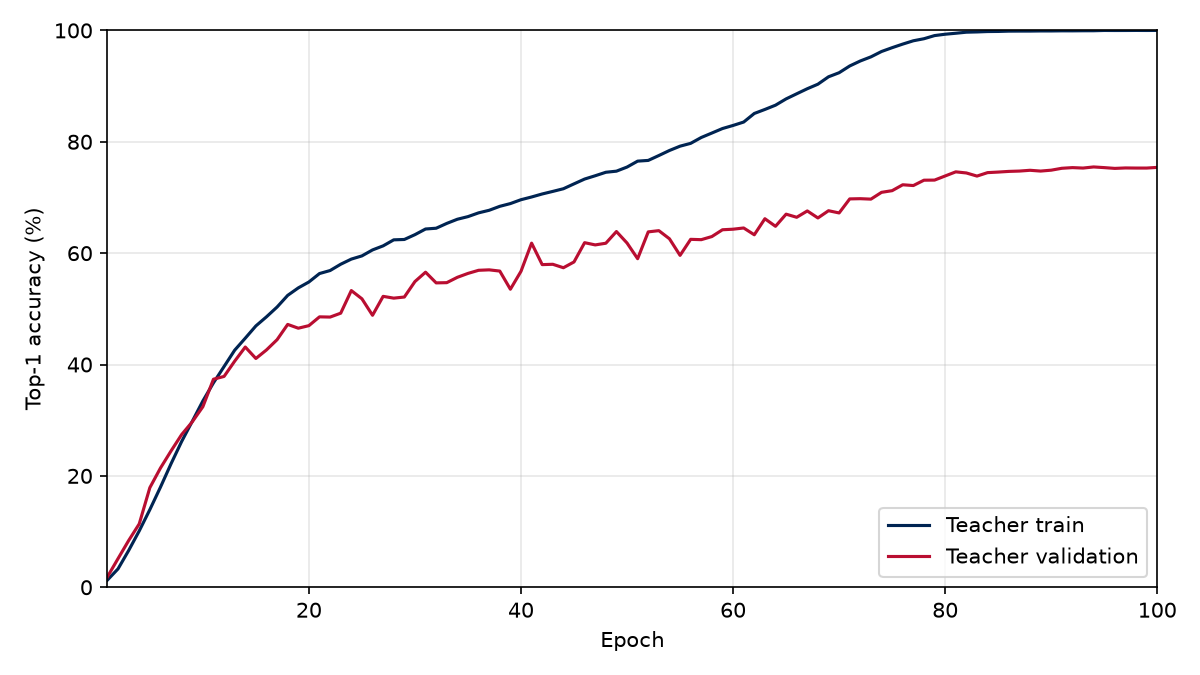
\includegraphics[width=0.85\linewidth]{results/teacher_training.png}%
  }{%
    \fbox{\parbox{0.85\linewidth}{\centering
      \textcolor{red}{[TODO: insert teacher training/validation curve graphic here
      (results/teacher\_training.png).]}}}%
  }
  \caption{Teacher training (blue) vs.\ validation (red) top-1 per epoch.
  Validation is still rising at epoch 100; best val 75.48 (epoch 94).}
  \label{fig:training}
\end{figure}

\subsection{Confusion matrix}

\begin{figure}[h]
  \centering
  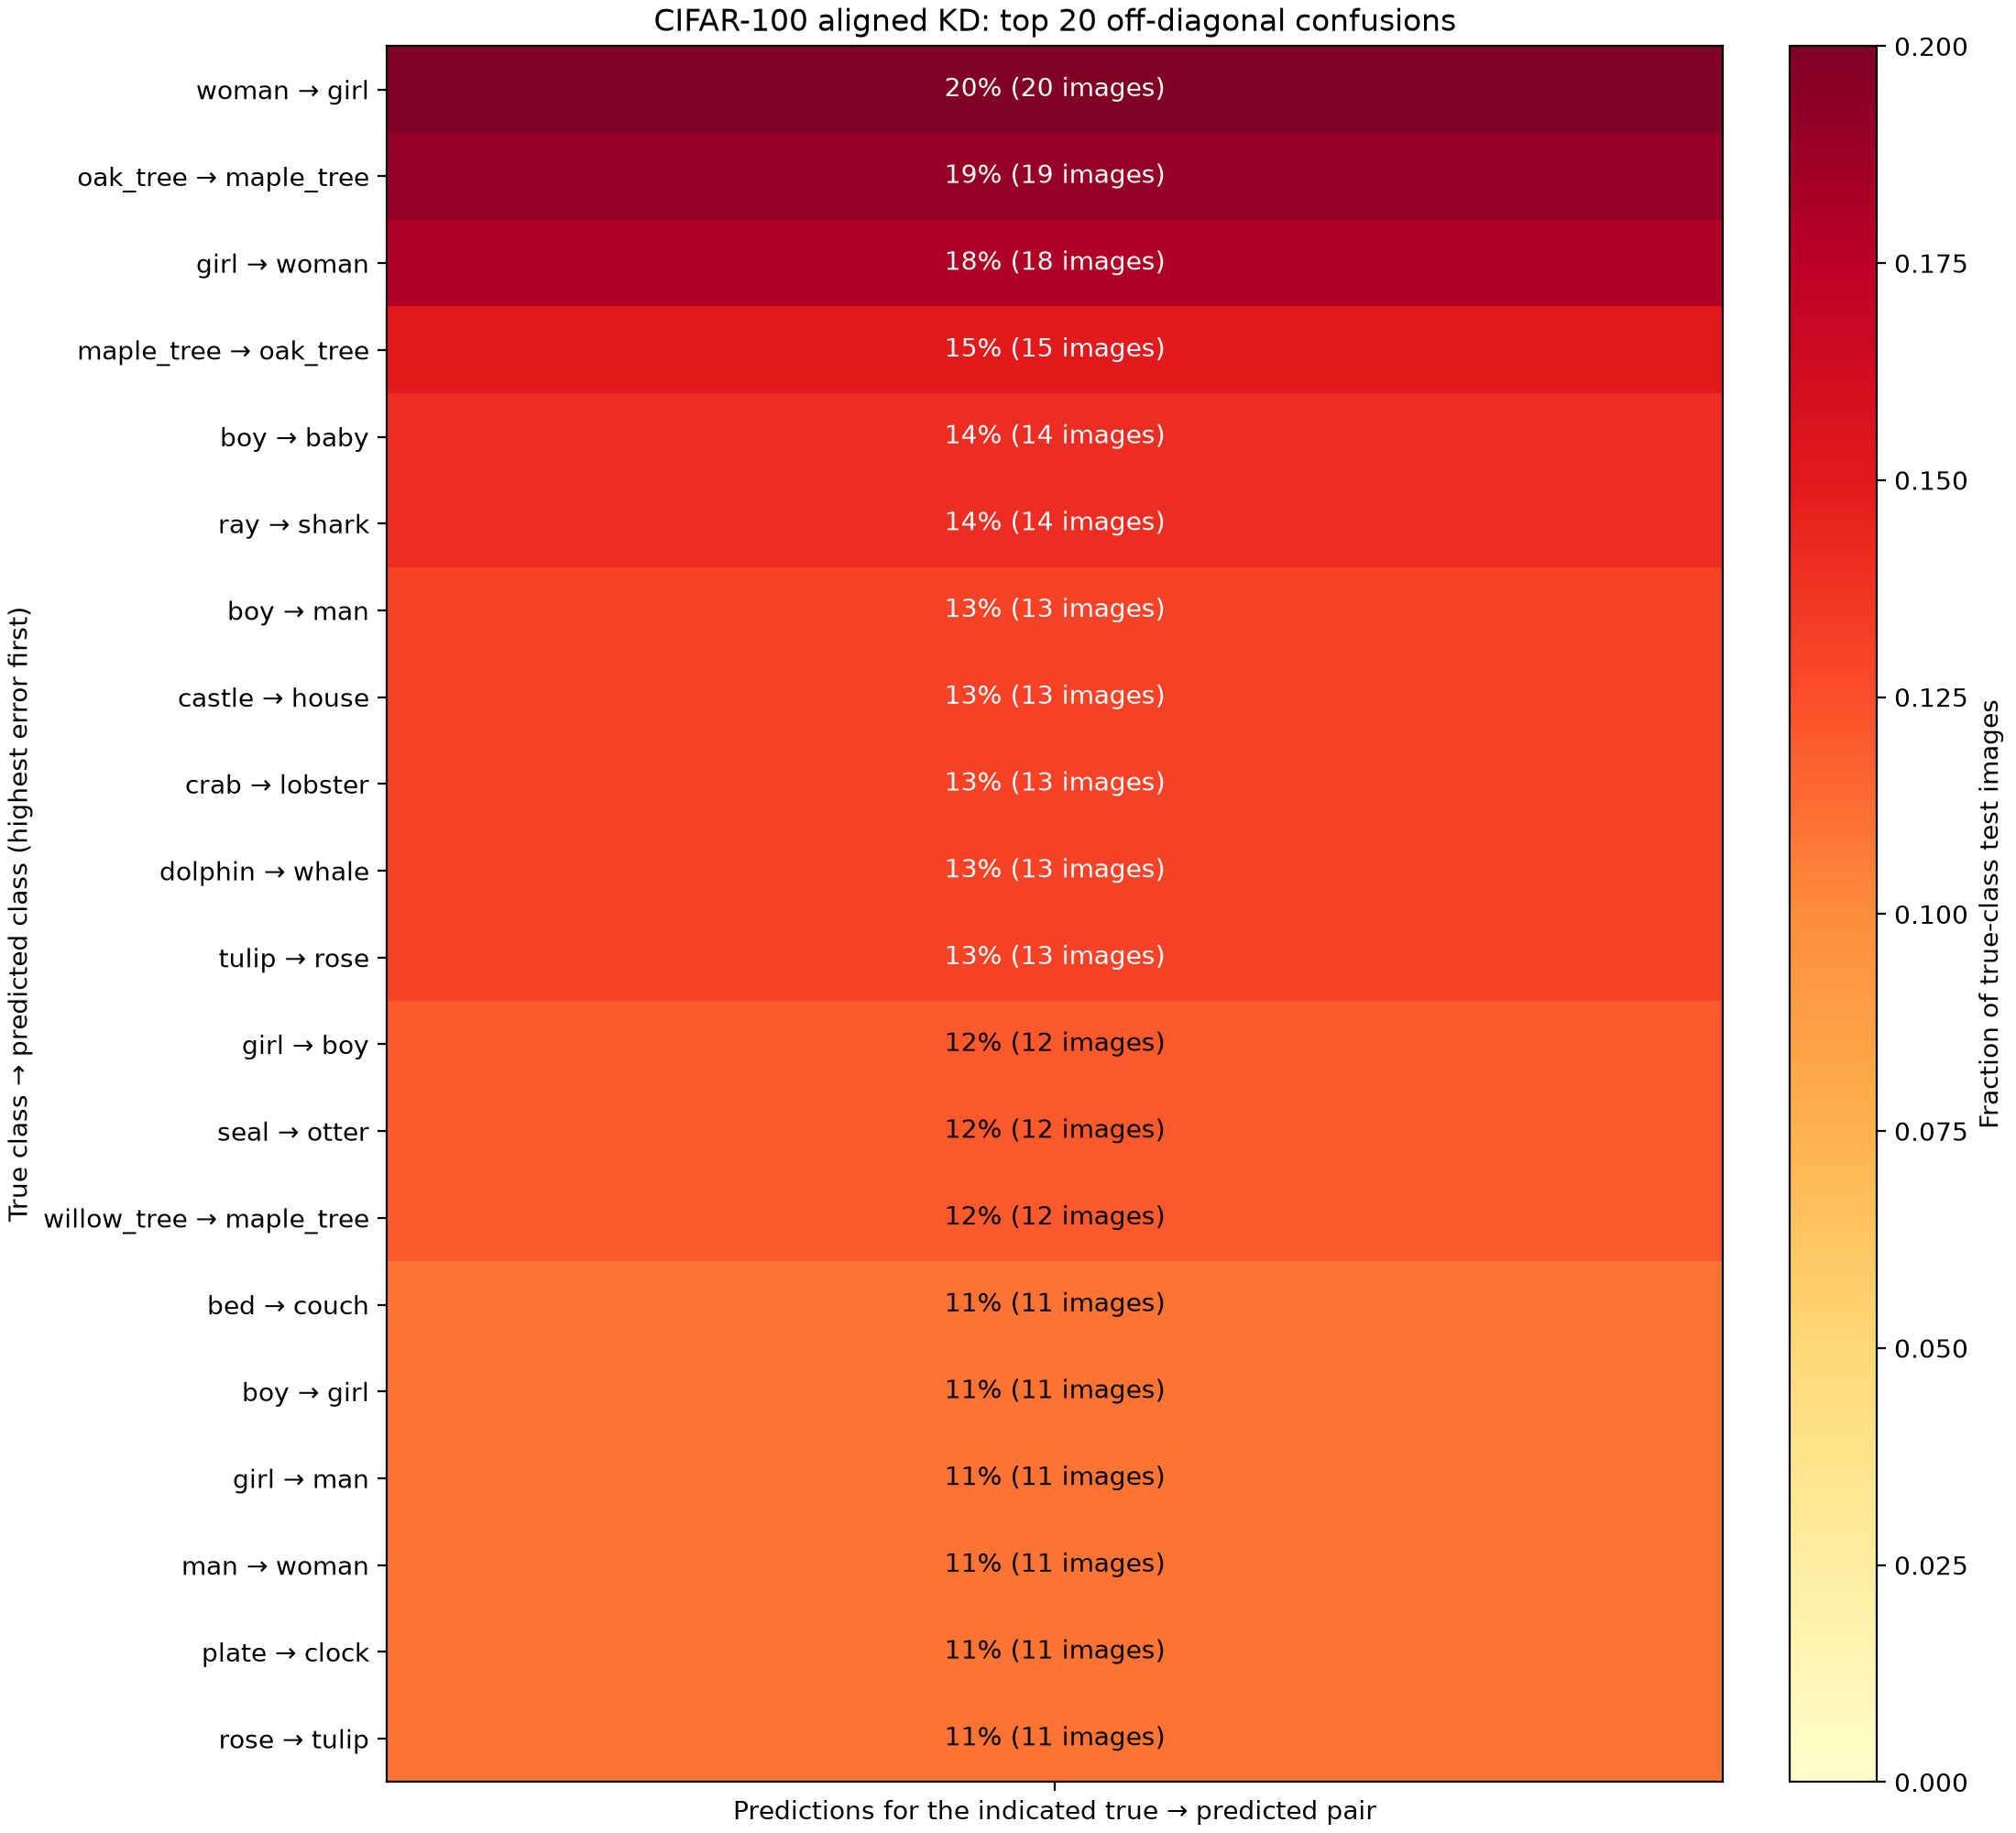
\includegraphics[width=0.75\linewidth]{results/confusion_matrix.png}
  \caption{Top-20 most-confused class pairs for the aligned KD student.
  The ten most frequent pairs are all within-superclass
  (\S\ref{sec:failure}); the remaining ten include a small number of
  cross-superclass errors such as plate$\to$clock.}
  \label{fig:confusion}
\end{figure}

\clearpage
\section{Appendix: Reproducibility Checklist}

\begin{itemize}[noitemsep]
  \item[$-$] README.md explains how to reproduce all main results with one
    command. \textcolor{red}{[TODO: expand README with quickstart.]}
  \item[$-$] requirements.txt lists dependencies with pinned versions.
    \textcolor{red}{[TODO: run \texttt{pip freeze >\allowbreak{} requirements.txt} before
    submission.]}
  \item[$\checkmark$] All random seeds are fixed and documented (split\_seed = 42).
  \item[$\times$] All results are mean $\pm$ std over $\geq$3 independent runs.
    \textit{Single seed (42) only; see \S\ref{sec:limitations}.}
  \item[$\checkmark$] GitHub repository is public and the link is in the report header
    (\url{https://github.com/l33zard/cakd}).
  \item[$\checkmark$] No hardcoded absolute paths in\\
    \texttt{scripts/\allowbreak{}evaluate\_test.py}
    or \texttt{scripts/\allowbreak{}cka\_diagnostic.py}.
  \item[$\checkmark$] Dataset is downloaded programmatically\\
    (\texttt{torchvision.datasets.\allowbreak{}CIFAR100(\allowbreak{}download=True)}).
  \item[$-$] Model checkpoints or inference instructions are included.
    \textcolor{red}{[TODO: link to Google Drive folder in README.]}
\end{itemize}

\end{document}
